% Options for packages loaded elsewhere
\PassOptionsToPackage{unicode}{hyperref}
\PassOptionsToPackage{hyphens}{url}
\PassOptionsToPackage{dvipsnames,svgnames,x11names}{xcolor}
%
\documentclass[
]{article}
\usepackage{amsmath,amssymb}
\usepackage{lmodern}
\usepackage{iftex}
\ifPDFTeX
  \usepackage[T1]{fontenc}
  \usepackage[utf8]{inputenc}
  \usepackage{textcomp} % provide euro and other symbols
\else % if luatex or xetex
  \usepackage{unicode-math}
  \defaultfontfeatures{Scale=MatchLowercase}
  \defaultfontfeatures[\rmfamily]{Ligatures=TeX,Scale=1}
\fi
% Use upquote if available, for straight quotes in verbatim environments
\IfFileExists{upquote.sty}{\usepackage{upquote}}{}
\IfFileExists{microtype.sty}{% use microtype if available
  \usepackage[]{microtype}
  \UseMicrotypeSet[protrusion]{basicmath} % disable protrusion for tt fonts
}{}
\makeatletter
\@ifundefined{KOMAClassName}{% if non-KOMA class
  \IfFileExists{parskip.sty}{%
    \usepackage{parskip}
  }{% else
    \setlength{\parindent}{0pt}
    \setlength{\parskip}{6pt plus 2pt minus 1pt}}
}{% if KOMA class
  \KOMAoptions{parskip=half}}
\makeatother
\usepackage{xcolor}
\IfFileExists{xurl.sty}{\usepackage{xurl}}{} % add URL line breaks if available
\IfFileExists{bookmark.sty}{\usepackage{bookmark}}{\usepackage{hyperref}}
\hypersetup{
  pdftitle={Technical comment on `Negative-assortative mating for color in wolves'},
  colorlinks=true,
  linkcolor={blue},
  filecolor={Maroon},
  citecolor={Blue},
  urlcolor={Blue},
  pdfcreator={LaTeX via pandoc}}
\urlstyle{same} % disable monospaced font for URLs
\usepackage[margin=1in]{geometry}
\usepackage{longtable,booktabs,array}
\usepackage{calc} % for calculating minipage widths
% Correct order of tables after \paragraph or \subparagraph
\usepackage{etoolbox}
\makeatletter
\patchcmd\longtable{\par}{\if@noskipsec\mbox{}\fi\par}{}{}
\makeatother
% Allow footnotes in longtable head/foot
\IfFileExists{footnotehyper.sty}{\usepackage{footnotehyper}}{\usepackage{footnote}}
\makesavenoteenv{longtable}
\usepackage{graphicx}
\makeatletter
\def\maxwidth{\ifdim\Gin@nat@width>\linewidth\linewidth\else\Gin@nat@width\fi}
\def\maxheight{\ifdim\Gin@nat@height>\textheight\textheight\else\Gin@nat@height\fi}
\makeatother
% Scale images if necessary, so that they will not overflow the page
% margins by default, and it is still possible to overwrite the defaults
% using explicit options in \includegraphics[width, height, ...]{}
\setkeys{Gin}{width=\maxwidth,height=\maxheight,keepaspectratio}
% Set default figure placement to htbp
\makeatletter
\def\fps@figure{htbp}
\makeatother
\setlength{\emergencystretch}{3em} % prevent overfull lines
\providecommand{\tightlist}{%
  \setlength{\itemsep}{0pt}\setlength{\parskip}{0pt}}
\setcounter{secnumdepth}{-\maxdimen} % remove section numbering
\newlength{\cslhangindent}
\setlength{\cslhangindent}{1.5em}
\newlength{\csllabelwidth}
\setlength{\csllabelwidth}{3em}
\newlength{\cslentryspacingunit} % times entry-spacing
\setlength{\cslentryspacingunit}{\parskip}
\newenvironment{CSLReferences}[2] % #1 hanging-ident, #2 entry spacing
 {% don't indent paragraphs
  \setlength{\parindent}{0pt}
  % turn on hanging indent if param 1 is 1
  \ifodd #1
  \let\oldpar\par
  \def\par{\hangindent=\cslhangindent\oldpar}
  \fi
  % set entry spacing
  \setlength{\parskip}{#2\cslentryspacingunit}
 }%
 {}
\usepackage{calc}
\newcommand{\CSLBlock}[1]{#1\hfill\break}
\newcommand{\CSLLeftMargin}[1]{\parbox[t]{\csllabelwidth}{#1}}
\newcommand{\CSLRightInline}[1]{\parbox[t]{\linewidth - \csllabelwidth}{#1}\break}
\newcommand{\CSLIndent}[1]{\hspace{\cslhangindent}#1}
\usepackage{setspace}
\onehalfspacing

\usepackage{lineno}
\linenumbers

\usepackage{amsmath}
\ifLuaTeX
  \usepackage{selnolig}  % disable illegal ligatures
\fi

\title{Technical comment on `Negative-assortative mating for color in wolves'}
\author{}
\date{\vspace{-2.5em}}

\begin{document}
\maketitle

\hypertarget{background}{%
\subsection{Background}\label{background}}

Hedrick et al. (\protect\hyperlink{ref-hedrick_negative-assortative_2016}{2016}) reported on ``negative-assortative mating for color in wolves'' from Yellowstone National Park, the ``first documented case of significant negative-assortative mating in mammals.'' Based on the close correspondence of genotype and allele frequencies observed in the wild to that predicted by their population genetic model, they conclude that ``negative-assortative mating could be entirely responsible for the maintenance of this well-known color polymorphism.'' While researching examples of nonrandom mating in the wild to teach in class I discovered that the results of their population genetic model are inconsistent with their stated assumptions, as I understand them. In this paper, I revisit the model with the following two objectives:

\begin{enumerate}
\def\labelenumi{\arabic{enumi}.}
\tightlist
\item
  Demonstrate that the frequency of negative-assortative mating between gray and black pelage color morphs in their model does not follow from their assumptions; and
\item
  Derive results that are consistent with their assumptions.
\end{enumerate}

I am critiquing only their model, not the data analysis or conclusions. Both the original model and the new model analyzed here lead to similar inferences about the maintenance of the pelage color polymorphism because the equilibrium genotype and allele frequencies are nearly the same in both models. However, it is important that the mathematical biology literature provide logically consistent analysis so that future researchers may benefit most from its insights.

\hypertarget{the-frequency-of-assortative-mating-is-inconsistent-with-the-assumptions}{%
\subsection{The frequency of assortative mating is inconsistent with the assumptions}\label{the-frequency-of-assortative-mating-is-inconsistent-with-the-assumptions}}

Hedrick et al. (\protect\hyperlink{ref-hedrick_negative-assortative_2016}{2016}) assume that a proportion \(A\) matings are assortative, but the proportion they derive is much less (see Fig. \ref{fig:sample-space} for a graphical derivation). For consistency, I use the same symbols as Hedrick et al. (\protect\hyperlink{ref-hedrick_negative-assortative_2016}{2016}) (Table \ref{tab:symbols} lists all symbols and their definitions). I infer three key assumptions from the two statements on the bottom-left of pg. 758 of Hedrick et al. (\protect\hyperlink{ref-hedrick_negative-assortative_2016}{2016}):

\begin{quote}
``gray wolves have a genotype of \(kk\) and an assumed frequency of \(P\) and black
wolves have genotypes \(Kk\) and \(KK\) with frequencies \(H\) and \(Q\), respectively \((P + H + Q = 1)\).''
\end{quote}

\begin{quote}
``Assume that \(A\) and \(1-A\) are the proportions of negative-assortative mating and random mating, respectively, in the population.''
\end{quote}

From these statements, I infer that:

\begin{enumerate}
\def\labelenumi{\arabic{enumi}.}
\tightlist
\item
  \(kk\), \(Kk\), and \(KK\) are mutually exclusive genotypes with frequencies \(P\), \(H\), and \(Q\)
\item
  Negative-assortative mating and random mating are mutually exclusive mating types with frequencies \(A\) and \(1-A\)
\item
  Genotype and mating type are independent (\(\mathrm{Pr}[A \cap B] = \mathrm{Pr}[A] \times \mathrm{Pr}[B]\))
\end{enumerate}

Other standard population genetic assumptions such as infinite population size also apply.

\begin{figure}[ht]
  \centering
  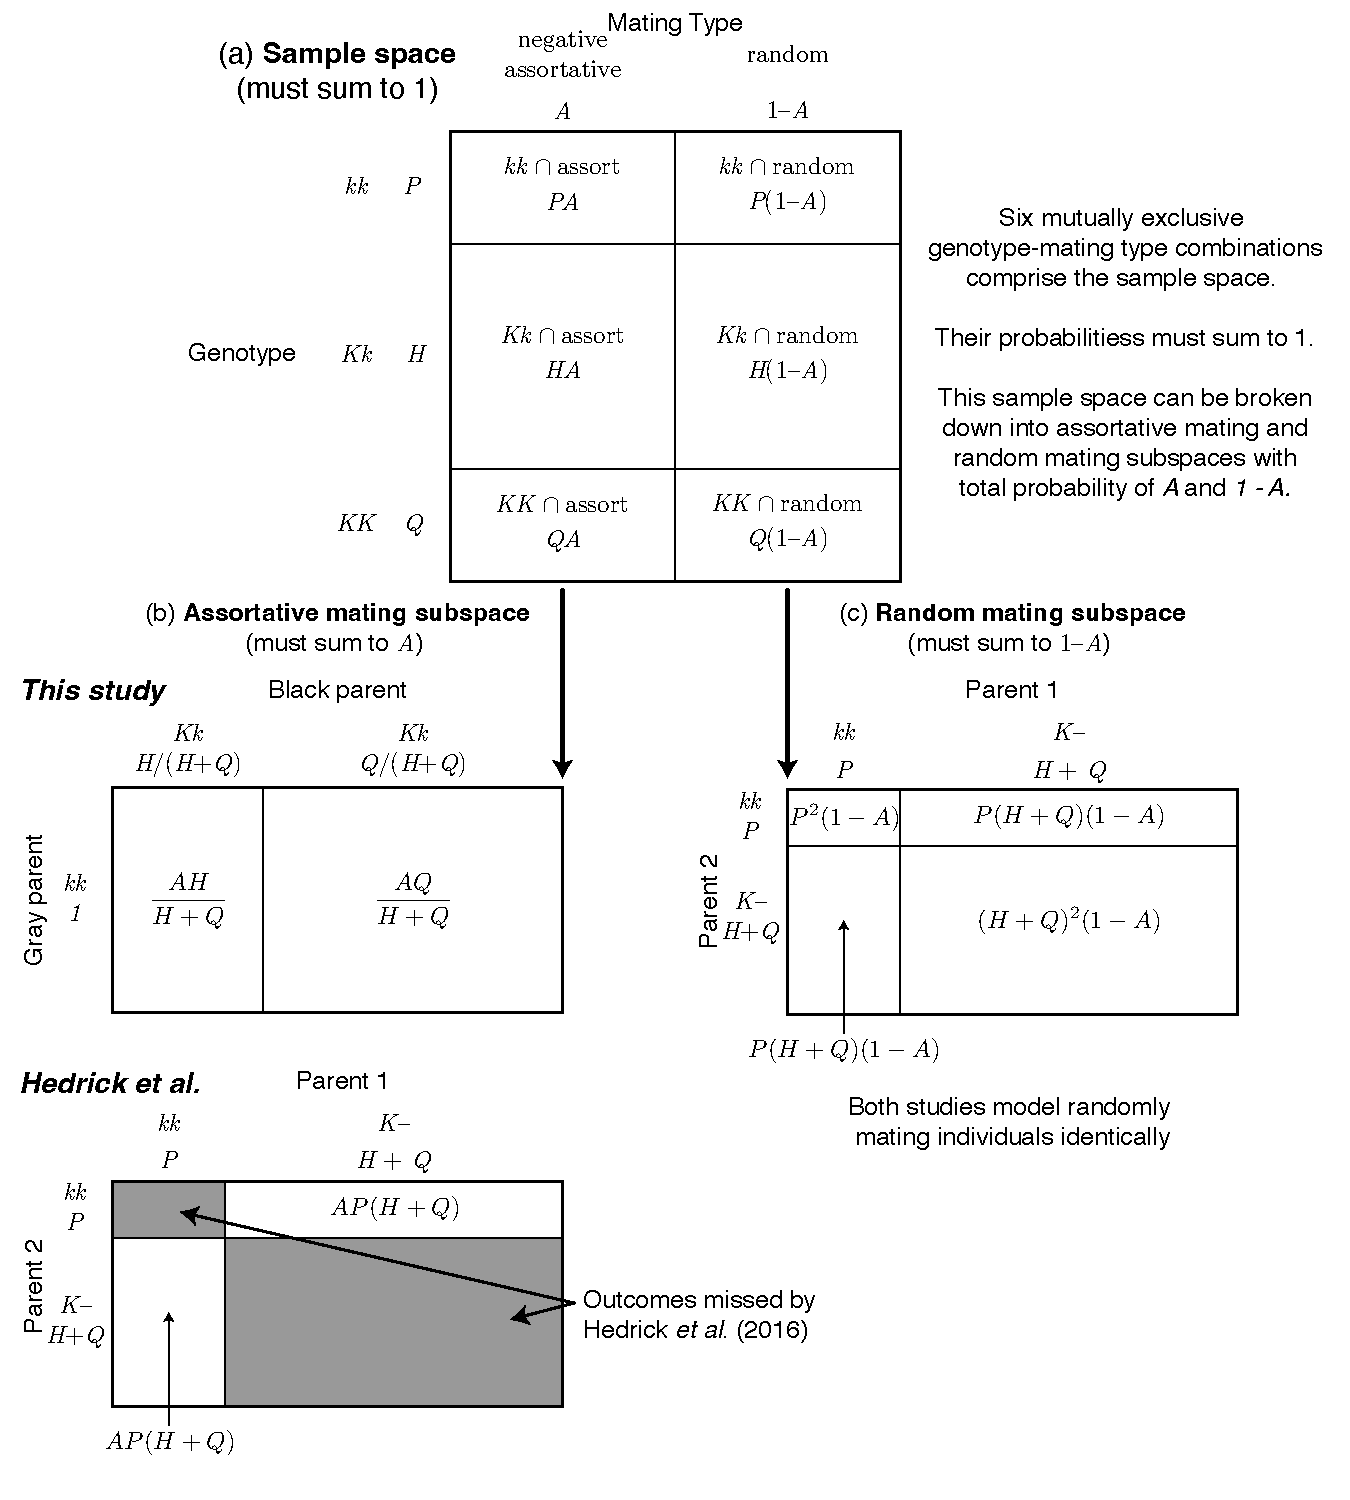
\includegraphics[width=\textwidth]{../figures/sample-space.pdf}
  \caption{(Caption next page.)}
  \label{fig:sample-space}
\end{figure}
\addtocounter{figure}{-1}

\begin{figure} [t!]
\caption{(Previous page.) A graphical summary of the sample space that illustrates why this model arrives at results that differ from Hedrick \textit{et al.} (2016). (a) The sample space consists of six mutually exclusive genotype-mating type combinations that must sum to 1 given the assumptions. (b) In this study we show that the the probabilities in the assortative mating subspace sum to $A$, as assumed, if one conditions on assortative mating consisting of a black and gray coat color parent. In contrast, Hedrick \textit{et al.} (2016) effectively assume that a proportion of assortatively mating individuals equal to the area of the gray boxes do not contribute matings. This is why the models reach different conclusions. (c) Both models treat randomly mating individuals identically.}
\end{figure}

\begin{longtable}[]{@{}ccl@{}}
\caption{\label{tab:symbols}Glossary of mathematical symbols, variable string used in source code, and description.}\tabularnewline
\toprule
Symbol & Variable string & Description \\
\midrule
\endfirsthead
\toprule
Symbol & Variable string & Description \\
\midrule
\endhead
\(k\) & \(\mathtt{k}\) & recessive beta-defensin variant \\
\(K\) & \(\mathtt{K}\) & dominant beta-defensin variant \\
\(p\) & \(\mathtt{p}\) & frequency of \(\textit{k}\) allele \\
\(q\) & \(\mathtt{q}\) & frequency of \(\textit{K}\) allele \\
\(P\) & \(\mathtt{P}\) & frequency of \(\textit{kk}\) genotype \\
\(H\) & \(\mathtt{H}\) & frequency of \(\textit{Kk}\) genotype \\
\(Q\) & \(\mathtt{Q}\) & frequency of \(\textit{KK}\) genotype \\
\(A\) & \(\mathtt{A}\) & proportion negative-assortatively mating \\
\bottomrule
\end{longtable}

Based on these assumptions, I deduce that:

\begin{enumerate}
\def\labelenumi{\arabic{enumi}.}
\tightlist
\item
  The probability of all genotype-mating type combinations must sum to 1
\item
  The probability of all genotypes in the assortative-mating subspace must sum to \(A\)
\item
  The probability of all genotypes in the random-mating subspace must sum to \(1-A\)
\end{enumerate}

There are six mutually exclusive genotype-mating type combinations in the population sample space (Fig. \ref{fig:sample-space}a). Since \(P+H+Q=1\), \(A + 1 - A = 1\), and genotype is independent of mating type, the probability of all genotype-mating type combinations must sum to 1.

\begin{multline*}
 \sum_i^{\{\mathit{kk}, \mathit{Kk}, \mathit{KK}\}} \sum_j^{\{\textrm{assort}, \textrm{random}\}} \textrm{Genotype}_i \cap \textrm{Mating~type}_j = \\  
  (\mathit{kk} \cap \textrm{assort}) + (\mathit{Kk} \cap \textrm{assort}) + 
  (\mathit{KK} \cap \textrm{assort}) + \\ (\mathit{kk} \cap \textrm{random}) + 
  (\mathit{Kk} \cap \textrm{random}) + (\mathit{KK} \cap \textrm{random}) \\
 = PA + HA + QA + P (1 - A) + H (1 - A) + Q (1 - A) \\
 = A (P + H + Q) + (1 - A) (P + H + Q) \\
 = 1 - A + A \\
 = 1 \\
\end{multline*}

Furthermore, we know that within the negative-assortative and random mating subspaces, the total probability must sum to \(A\) and \(1 - A\), respectively:

\begin{align*}
  A = & PA + HA + QA \\
  1 - A = & P (1 - A) + H (1 - A) + Q (1 - A)
\end{align*}
The model in Hedrick et al. (\protect\hyperlink{ref-hedrick_negative-assortative_2016}{2016}) is internally inconsistent because the proportion of negative-assortative matings does not equal \(A\) as defined (Fig. \ref{fig:sample-space}b).
\[A := \frac{\textrm{Assortative matings}}{\textrm{Total matings}} =\frac{\textrm{Assortative matings}}{\textrm{Assortative} + \textrm{Random matings}}\]
Hedrick et al. (\protect\hyperlink{ref-hedrick_negative-assortative_2016}{2016}) state that the frequency of assortative matings is \(2 A P (H + Q)\) (\emph{cf} top of pg. 759) and the frequency of random matings is \(1 - A\). Applying these frequencies reveals that the proportion of assortative matings is not equal to \(A\) as assumed:
\[ \frac{\textrm{Assortative matings}}{\textrm{Assortative} + \textrm{Random matings}} = \frac{2 A P (H + Q)}{2 A P (H + Q) + 1 - A}\]
There are no solutions to the expression above where the proportion of negative-assortative mating would equal \(A\) when genotype and mating proportions are between 0 and 1. With their model, the actual proportion of negative-assortative would vary from 0 when \(P = 0\) or \(P = 1\) and \(A / (2 - A)\) when \(P = 0.5\).

To summarize, a proportion \(A\) should mate assortatively given the assumptions of their model, but only \(2 AP(H+Q)\) actually mate assortatively according to their results. In essence, they assign a proportion \(A\) to mate assortatively, but then a proportion \(A - 2 AP(H+Q)\) do not mate assortatively (the area of the gray regions in Fig. \ref{fig:sample-space}b), and are therefore not counted among the total number of matings. This is why the probabilities of all matings do not sum to 1. The logically consistent solution is to condition on the fact that if a mating is negative-assortative it must by definition have one gray and one black parent (Fig. \ref{fig:sample-space}b). In the next section, I use this approach to derive new results. In contrast, Hedrick et al. (\protect\hyperlink{ref-hedrick_negative-assortative_2016}{2016}) effectively impose selection without ever stating that assumption. To deal with the fact that resulting genotype frequencies do not sum to 1, they regularize the frequencies (\emph{cf} equation 1a-b), as normally done in models of selection. Regularization is appropriate with selection because selection shrinks or expands the sample space as long as average fitness does not equal 1. Hedrick et al. (\protect\hyperlink{ref-hedrick_negative-assortative_2016}{2016}) impose selection because some of the assortative-mating individuals do not mate assortatively and are therefore not counted among the matings that result in offspring.

\hypertarget{revised-solutions-consistent-with-model-assumptions}{%
\subsection{Revised solutions consistent with model assumptions}\label{revised-solutions-consistent-with-model-assumptions}}

The previous section showed that the frequency of assortative gray \(\times\) black matings was not derived in a manner logically consistent with the model's assumptions. Here I derive new mating frequencies, genotype frequencies, and equilibria. I used Sympy version 1.7.1 (\protect\hyperlink{ref-meurer_sympy:_2017}{Meurer et al. 2017}) for symbolic derivations through Python version 3.6 and the \emph{R} package \textbf{reticulate} version 1.25 (\protect\hyperlink{ref-ushey_reticulate_2022}{Ushey et al. 2022}). All other computations were performed in \emph{R} version 4.2.0 (\protect\hyperlink{ref-r_core_team_r:_2022}{R Core Team 2022}). The source code is available in a public GitHub repository and will be archived on Zenodo upon publication.

Table \ref{tab:probabilities} derives the probabilities of all possible outcomes and Table \ref{tab:genotypes} summarizes the frequency each mating combination. This is the exact same process used to derive frequency of mating combinations in positive-assortative mating models (e.g. \protect\hyperlink{ref-hedrick_population_2012}{Hedrick and Ritland 2012}). Since I model random mating identically to the previous model, the frequencies of gray \(\times\) gray and black \(\times\) black matings are identical; only the frequency of gray \(\times\) black matings differs between models (Table \ref{tab:genotypes}; Fig. @ref\{fig:sample-space\}c).

Code in the Supporting Information derives the expressions in (Table \ref{tab:genotypes}) analytically using a computer algebra system, but one can also use the Law of Total Probability to prove it. The Law of Total Probability for discrete probability distributions states that \(\mathrm{Pr}[A] = \sum_i \mathrm{Pr}[A|B_i] \mathrm{Pr}[B_i]\) where \(\mathrm{Pr}[A|B_i]\) is the probability of outcome \(A\) conditional on outcome \(B_i\). The total probability of \(A\) is the sum of conditional probabilities across all outcomes for event \(B\). Using the Law of Total Probability, the probability of a gray \(\times\) black mating is:
\[\mathrm{Pr}[\textrm{gray} \times \textrm{black}] = \mathrm{Pr}[\textrm{gray} \times \textrm{black}|\textrm{assort}] \mathrm{Pr}[\textrm{assort}] + \mathrm{Pr}[\textrm{gray} \times \textrm{black}|\textrm{random}] \mathrm{Pr}[\textrm{random}]\]
We already assume that \(\mathrm{Pr}[\textrm{assort}] = A\) and \(\mathrm{Pr}[\textrm{random}] = 1 - A\). With random mating, I arrive at the same expression as Hedrick et al. (\protect\hyperlink{ref-hedrick_negative-assortative_2016}{2016}), \(\mathrm{Pr}[\textrm{gray} \times \textrm{black}|\textrm{random}] = 2P(H+Q)\) (\emph{cf} top of pg. 759). If the mating is negative-assortative, then it \emph{must} be a gray \(\times\) black mating. Therefore, \(\mathrm{Pr}[\textrm{gray} \times \textrm{black}|\textrm{assort}] = 1\). Putting these together, I obtain:

\begin{align*}
  \mathrm{Pr}[\textrm{gray} \times \textrm{black}] = & 1 \times A + 2P(H+Q) \times (1-A) \\
  = & A + 2 P (H + Q) (1 - A)
\end{align*}

This result diverges from that given in Hedrick et al. (\protect\hyperlink{ref-hedrick_negative-assortative_2016}{2016}), where they report the frequency of gray \(\times\) black matings is \(2 P (H + Q)\) (\emph{cf} Table 1).

\begin{longtable}[]{@{}
  >{\raggedright\arraybackslash}p{(\columnwidth - 14\tabcolsep) * \real{0.0833}}
  >{\raggedright\arraybackslash}p{(\columnwidth - 14\tabcolsep) * \real{0.1204}}
  >{\raggedright\arraybackslash}p{(\columnwidth - 14\tabcolsep) * \real{0.1111}}
  >{\raggedright\arraybackslash}p{(\columnwidth - 14\tabcolsep) * \real{0.1019}}
  >{\raggedright\arraybackslash}p{(\columnwidth - 14\tabcolsep) * \real{0.0833}}
  >{\raggedright\arraybackslash}p{(\columnwidth - 14\tabcolsep) * \real{0.1204}}
  >{\raggedright\arraybackslash}p{(\columnwidth - 14\tabcolsep) * \real{0.1852}}
  >{\raggedright\arraybackslash}p{(\columnwidth - 14\tabcolsep) * \real{0.1944}}@{}}
\caption{\label{tab:probabilities}The probability of every mating outcome in the negative-assortative mating model analyzed by Hedrick \emph{et al.} (2016). For the notation, the probability of event \emph{X} is Pr{[}\emph{X}{]}. The total probabilities for each row are derived from the product of all probabilities in the same row, Pr{[}Total{]} = Pr{[}Parent 1{]} \(\times\) Pr{[}Mating{]} \(\times\) Pr{[}Parent 2{]}.}\tabularnewline
\toprule
\begin{minipage}[b]{\linewidth}\raggedright
Parent 1
\end{minipage} & \begin{minipage}[b]{\linewidth}\raggedright
Pr{[}Parent 1{]}
\end{minipage} & \begin{minipage}[b]{\linewidth}\raggedright
Mating
\end{minipage} & \begin{minipage}[b]{\linewidth}\raggedright
Pr{[}Mating{]}
\end{minipage} & \begin{minipage}[b]{\linewidth}\raggedright
Parent 2
\end{minipage} & \begin{minipage}[b]{\linewidth}\raggedright
Pr{[}Parent 2{]}
\end{minipage} & \begin{minipage}[b]{\linewidth}\raggedright
Pr{[}Total{]}
\end{minipage} & \begin{minipage}[b]{\linewidth}\raggedright
Color
\end{minipage} \\
\midrule
\endfirsthead
\toprule
\begin{minipage}[b]{\linewidth}\raggedright
Parent 1
\end{minipage} & \begin{minipage}[b]{\linewidth}\raggedright
Pr{[}Parent 1{]}
\end{minipage} & \begin{minipage}[b]{\linewidth}\raggedright
Mating
\end{minipage} & \begin{minipage}[b]{\linewidth}\raggedright
Pr{[}Mating{]}
\end{minipage} & \begin{minipage}[b]{\linewidth}\raggedright
Parent 2
\end{minipage} & \begin{minipage}[b]{\linewidth}\raggedright
Pr{[}Parent 2{]}
\end{minipage} & \begin{minipage}[b]{\linewidth}\raggedright
Pr{[}Total{]}
\end{minipage} & \begin{minipage}[b]{\linewidth}\raggedright
Color
\end{minipage} \\
\midrule
\endhead
\(kk\) & \(P\) & assortative & \(A\) & \(kk\) & \(0\) & \(0\) & Gray \(\times\) gray \\
\(kk\) & \(P\) & random & \(1 - A\) & \(kk\) & \(P\) & \(P^2 (1 - A)\) & Gray \(\times\) gray \\
\(kk\) & \(P\) & assortative & \(A\) & \(K-\) & \(1\) & \(AP\) & Gray \(\times\) black \\
\(kk\) & \(P\) & random & \(1 - A\) & \(K-\) & \(H + Q\) & \(P (H + Q) (1 - A)\) & Gray \(\times\) black \\
\(K-\) & \(H + Q\) & assortative & \(A\) & \(kk\) & \(1\) & \(A (H + Q)\) & Gray \(\times\) black \\
\(K-\) & \(H + Q\) & random & \(1 - A\) & \(kk\) & \(P\) & \(P (H + Q) (1 - A)\) & Gray \(\times\) black \\
\(K-\) & \(H + Q\) & assortative & \(A\) & \(K-\) & \(0\) & \(0\) & Black \(\times\) black \\
\(K-\) & \(H + Q\) & random & \(1 - A\) & \(K-\) & \(H + Q\) & \((H + Q)^2 (1 - A)\) & Black \(\times\) black \\
\bottomrule
\end{longtable}

\begin{longtable}[]{@{}
  >{\raggedright\arraybackslash}p{(\columnwidth - 6\tabcolsep) * \real{0.2143}}
  >{\raggedright\arraybackslash}p{(\columnwidth - 6\tabcolsep) * \real{0.1735}}
  >{\raggedright\arraybackslash}p{(\columnwidth - 6\tabcolsep) * \real{0.3469}}
  >{\raggedright\arraybackslash}p{(\columnwidth - 6\tabcolsep) * \real{0.2653}}@{}}
\caption{\label{tab:genotypes}Hedrick \emph{et al.} (2016) incorrectly derive the frequency of gray \(\times\) black. The corrected expressions are provided here.}\tabularnewline
\toprule
\begin{minipage}[b]{\linewidth}\raggedright
Color
\end{minipage} & \begin{minipage}[b]{\linewidth}\raggedright
Mating Genotypes
\end{minipage} & \begin{minipage}[b]{\linewidth}\raggedright
Frequency (Hedrick \emph{et al.} 2016)
\end{minipage} & \begin{minipage}[b]{\linewidth}\raggedright
Frequency (this paper)
\end{minipage} \\
\midrule
\endfirsthead
\toprule
\begin{minipage}[b]{\linewidth}\raggedright
Color
\end{minipage} & \begin{minipage}[b]{\linewidth}\raggedright
Mating Genotypes
\end{minipage} & \begin{minipage}[b]{\linewidth}\raggedright
Frequency (Hedrick \emph{et al.} 2016)
\end{minipage} & \begin{minipage}[b]{\linewidth}\raggedright
Frequency (this paper)
\end{minipage} \\
\midrule
\endhead
Gray \(\times\) gray & \(kk \times kk\) & \(P^2 (1 - A)\) & \(P^2 (1 - A)\) \\
Gray \(\times\) black & \(kk \times K-\) & \(2 P (H + Q)\) & \(A + 2 P (H + Q) (1 - A)\) \\
Black \(\times\) black & \(K- \times K-\) & \((H + Q) ^ 2 (1 - A)\) & \((H + Q) ^ 2 (1 - A)\) \\
\bottomrule
\end{longtable}

Despite the different frequency of gray \(\times\) black matings resulting from each model, the equilibrium genotype frequencies are very similar. In both models, \(\hat{P} = 0.5\), implying \(0.5 = \hat{H} + \hat{Q}\). I find that \(\hat{Q} = (A / 2 - \sqrt{2 (A + 1)} + 1.5)/(1 - A)\), which is close to the equilibrium values obtained in Hedrick et al. (\protect\hyperlink{ref-hedrick_negative-assortative_2016}{2016}) through recursion (Fig. \ref{fig:fig2}). Next, I compared allele frequency change depicted in Figs. 3-4 of Hedrick et al. (\protect\hyperlink{ref-hedrick_negative-assortative_2016}{2016}) to that predicted with the new model. The effect of \(A\) on change in the frequency of the \(K\) allele is qualitatively similar, but much faster with the new model (Fig. \ref{fig:fig3}). This is because the magnitude of allele frequency change far from the equilibrium is much greater with the new model (Fig. \ref{fig:fig4}). As a result, Hedrick et al. (\protect\hyperlink{ref-hedrick_negative-assortative_2016}{2016}) overestimate how long it would take for \(K\) to reach equilibrium given observed levels of assortative mating (\(A = 0.430\)). They conclude that \(K\) would reach equilibrium at \(\hat{q} = 0.278\) in 25 generations with \(A = 0.430\). In the revised model, \(K\) would reach equilibrium at \(\hat{q} = 0.271\) in only 15 generations with \(A = 0.430\) and a starting allele frequency \(q_0 = 0.01\). Hence, the revised model actually lends credence to their conclusion that negative-assortative mating may be a better explanation than heterozygote advantage for variation at the beta definsin locus.

\begin{figure}

{\centering 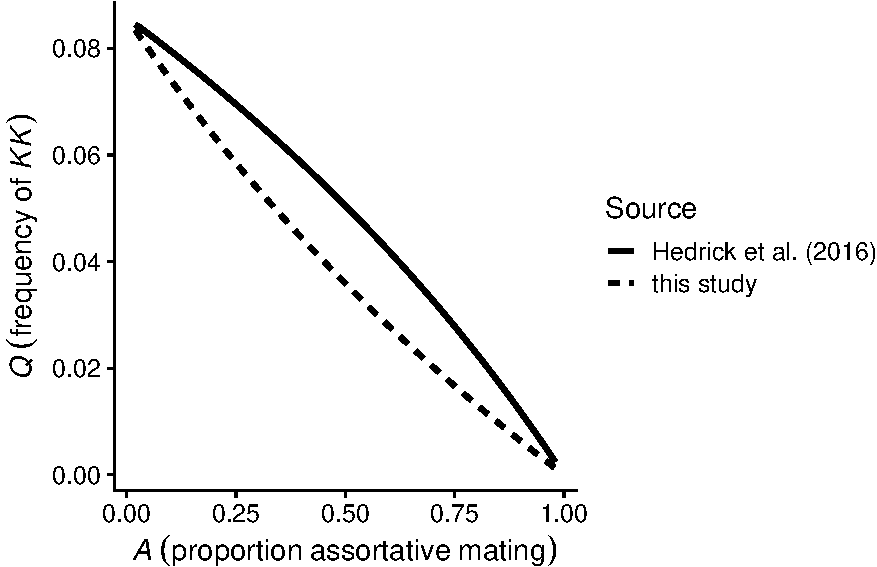
\includegraphics{ms_files/figure-latex/fig2-1} 

}

\caption{The equilibirum frequency of $Q$, the $\mathit{KK}$ homozygote in this study (dashed line) and Hedrick \textit{et al.} (2016) (solid line) for possible values of $A$, the proportion of wolves mating assortatively by color.}\label{fig:fig2}
\end{figure}

\begin{figure}[ht]
  \centering
  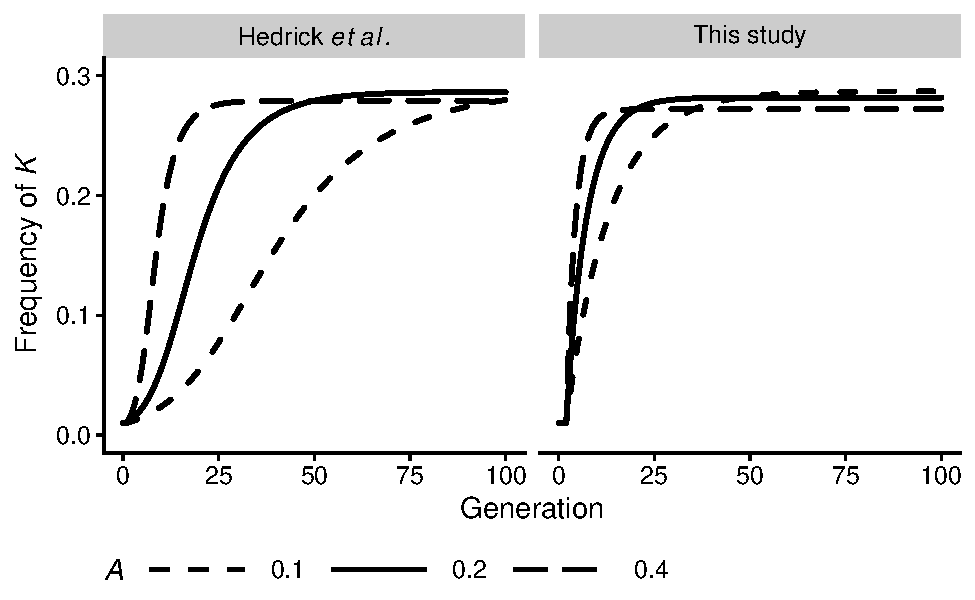
\includegraphics[width=\textwidth]{../figures/fig3.pdf}
  \caption{A comparison of the change in frequency of the black allele $K$ between Hedrick \textit{et al.} (2016) and this study. $K$ starts at a frequency 0.01 and the plots show the dynamics for three different levels of negative-assortative mating $A$.}
  \label{fig:fig3}
\end{figure}

\begin{figure}[ht]
  \centering
  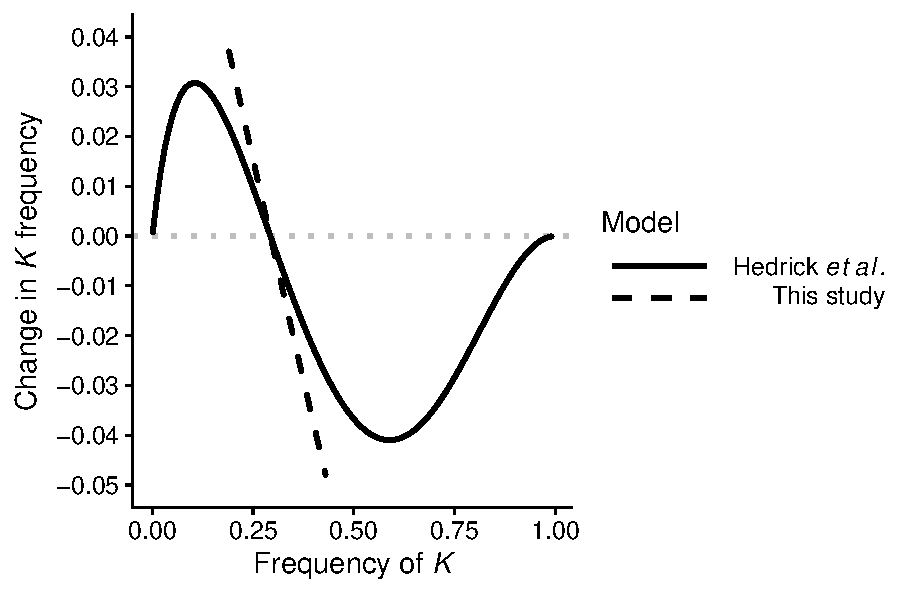
\includegraphics[width=\textwidth]{../figures/fig4.pdf}
  \caption{A comparison of the change in frequency of the black allele $K$ between Hedrick \textit{et al.} (2016) and this study. The initial frequency of $K$ is along the $x$-axis and the change in $K$ along the $y$-axis where $A = 0.430$ as in Hedrick \textit{et al.} (2016) Fig. 4. The models have the similar equilibrua where they cross the gray dotted line at 0, but in this study the magnitude of change in allele frequency increases the system gets further from this equilibrium.}
  \label{fig:fig4}
\end{figure}

In conclusion, the logical inconsistency in Hedrick et al. (\protect\hyperlink{ref-hedrick_negative-assortative_2016}{2016}) does not undermine their primary conclusion that negative-assortative mating by color may explain the distribution of genotype frequencies at the beta definsin locus in the Yellowstone population of wolves (\emph{Canis lupus}). The new derivation here may prove useful to future research on negative-assortative mating.

\hypertarget{literature-cited}{%
\section*{Literature cited}\label{literature-cited}}
\addcontentsline{toc}{section}{Literature cited}

\hypertarget{refs}{}
\begin{CSLReferences}{1}{0}
\leavevmode\vadjust pre{\hypertarget{ref-hedrick_population_2012}{}}%
Hedrick, P. W., and K. Ritland. 2012. \href{https://doi.org/10.1111/j.1558-5646.2011.01463.x}{Population genetics of the white-phased "{Spirit}" bear of {British} {Columbia}}. Evolution 66:305--313.

\leavevmode\vadjust pre{\hypertarget{ref-hedrick_negative-assortative_2016}{}}%
Hedrick, P. W., D. W. Smith, and D. R. Stahler. 2016. \href{https://doi.org/10.1111/evo.12906}{Negative-assortative mating for color in wolves}. Evolution 70:757--766.

\leavevmode\vadjust pre{\hypertarget{ref-meurer_sympy:_2017}{}}%
Meurer, A., C. P. Smith, M. Paprocki, O. Čertík, S. B. Kirpichev, M. Rocklin, A. Kumar, S. Ivanov, J. K. Moore, S. Singh, T. Rathnayake, S. Vig, B. E. Granger, R. P. Muller, F. Bonazzi, H. Gupta, S. Vats, F. Johansson, F. Pedregosa, M. J. Curry, A. R. Terrel, Š. Roučka, A. Saboo, I. Fernando, S. Kulal, R. Cimrman, and A. Scopatz. 2017. \href{https://doi.org/10.7717/peerj-cs.103}{{SymPy}: Symbolic computing in {Python}}. PeerJ Computer Science 3:e103.

\leavevmode\vadjust pre{\hypertarget{ref-r_core_team_r:_2022}{}}%
R Core Team. 2022. \href{http://www.R-project.org/}{R: {A} {Language} and {Environment} for {Statistical} {Computing}}. R Foundation for Statistical Computing, Vienna, Austria.

\leavevmode\vadjust pre{\hypertarget{ref-ushey_reticulate_2022}{}}%
Ushey, K., J. J. Allaire, and Y. Tang. 2022. \href{https://CRAN.R-project.org/package=reticulate}{Reticulate: {Interface} to '{Python}'}.

\end{CSLReferences}

\end{document}
